% % % % % % % % % % % % % % % % % % % % % % % % % % % % % % % % % % % % % % % % % % % % % % % % % % % % % % % % % % % % %
%
% Class Options (see http://www.brian-amberg.de/uni/poster/baposter/baposter_guide.pdf for more details)
%
% % % % % % % % % % % % % % % % % % % % % % % % % % % % % % % % % % % % % % % % % % % % % % % % % % % % % % % % % % % % %
% a0paper               % paper size (choose one)
% a1paper               %
% a2paper               %
% a3paper               %
% a4paper               %
% archE                 %
%
% paperwidth = length   % alternative to paper size eg paperwidth=100cm
% paperheight = length  %
%
% landscape             % paper orientation (choose one)
% portrait              %       
%
% margin = length       % give length e.g. margin=2cm
%
% fontscale = number    % font size
%
% showframe             % frame for debugging
%
% % % % % % % % % % % % % % % % % % % % % % % % % % % % % % % % % % % % % % % % % % % % % % % % % % % % % % % % % % % % %
\documentclass[a0paper,portrait,fontscale=0.3]{baposter}
\usepackage{graphicx} %to insert pictures
\usepackage{color} %to set colors
\usepackage{helvet} %to use helvet font
\usepackage{epstopdf}%convert eps files to pdf
\usepackage{calc}
\usepackage{graphicx}
\usepackage{amsmath}
\usepackage{amssymb}
\usepackage{relsize}
\usepackage{multirow}
\usepackage{rotating}
\usepackage{bm}
\usepackage{url}
\usepackage{caption}
\usepackage{multicol}
\usepackage{wrapfig}
\usepackage{subfig}
\usepackage{pgf}
\usepackage{enumitem}

%\usepackage{times}
%\usepackage{bookman}
\usepackage{palatino}

% \newcommand{\captionfont}{\footnotesize}

\graphicspath{{images/}{../images/}}
\usetikzlibrary{calc}

\newcommand{\SET}[1]  {\ensuremath{\mathcal{#1}}}
\newcommand{\MAT}[1]  {\ensuremath{\boldsymbol{#1}}}
\newcommand{\VEC}[1]  {\ensuremath{\boldsymbol{#1}}}
\newcommand{\Video}{\SET{V}}
\newcommand{\video}{\VEC{f}}
\newcommand{\track}{x}
\newcommand{\Track}{\SET T}
\newcommand{\LMs}{\SET L}
\newcommand{\lm}{l}
\newcommand{\PosE}{\SET P}
\newcommand{\posE}{\VEC p}
\newcommand{\negE}{\VEC n}
\newcommand{\NegE}{\SET N}
\newcommand{\Occluded}{\SET O}
\newcommand{\occluded}{o}
\renewcommand{\familydefault}{\sfdefault} %set default font to sans-serif for entire document.

%%%%%%%%%%%%%%%%%%%%%%%%%%%%%%%%%%%%%%%%%%%%%%%%%%%%%%%%%%%%%%%%%%%%%%%%%%%%%%%%
%%%% Some math symbols used in the text
%%%%%%%%%%%%%%%%%%%%%%%%%%%%%%%%%%%%%%%%%%%%%%%%%%%%%%%%%%%%%%%%%%%%%%%%%%%%%%%%

\newenvironment{alist}
{\renewcommand{\theenumi}{\alph{enumi}}
\renewcommand{\labelenumi}{\textup{(\theenumi)}}
\renewcommand{\theenumii}{\roman{enumii}}
\renewcommand{\labelenumii}{\textup{(\theenumii)}}
\begin{enumerate}}
{\end{enumerate}}

\newenvironment{rlist}
{\renewcommand{\theenumi}{\roman{enumi}}
\renewcommand{\labelenumi}{\textup{(\theenumi)}}
\begin{enumerate}}
{\end{enumerate}}

\newcommand{\dummy}[1]{\newcounter{#1}\setcounter{#1}{\value{enumii}}}
\newcommand{\rref}[1]{\tu{(\roman{#1})}}
\newcommand{\HRule}{\rule{\linewidth}{0.5mm}}

%choose one or other:
\newcommand{\lab}[1]{\label{#1} \quad #1\quad}%annotates equations
%\newcommand{\lab}[1]{\label{#1}}
%%%%%%
\newcommand{\ben}{\begin{enumerate}}
\newcommand{\een}{\end{enumerate}}
\newcommand{\be}{\begin{equation}}
\newcommand{\ee}{\end{equation}}
\newcommand{\bdm}{\begin{displaymath}}
\newcommand{\edm}{\end{displaymath}}
\newcommand{\bea}{\begin{eqnarray}}
\newcommand{\eea}{\end{eqnarray}}
\let\oldhat\hat
\renewcommand{\vec}[1]{\mathbf{#1}}
\renewcommand{\hat}[1]{\oldhat{\mathbf{#1}}}
\newcommand{\h}{\hspace{0.1in}}
\newcommand{\vsp}{\vspace*{0.2in}}
\newcommand{\tab}{\hspace{0.8in}}
\newcommand{\no}{\noindent}
\newcommand{\non}{\nonumber}
\newcommand{\pvint}{-\hspace{-1.1em}\int}%ordinary pv int after symbol
\newcommand{\bpvint}{-\hspace{-1em}\int}%pvint after bracket
\newcommand{\marg}{\marginpar}
\newcommand{\real}{\mbox{Re\,}}
\newcommand{\realnos}{\mbox{{\bf R}}}
\newcommand{\complexnos}{\mbox{{\bf C}}}
\newcommand{\integers}{\mbox{{\bf Z}}}
\newcommand{\naturalnos}{\mbox{{\bf N}}}
\newcommand{\rationalnos}{\mbox{{\bf Q}}}
\newcommand{\pdtwo}[2]{\frac{\partial ^{2} {#1}}{\partial{#2}^{2}}}
\newcommand{\pdone}[2]{\frac{\partial {#1}}{\partial {#2}}}
\newcommand{\sdone}[2]{\frac{d {#1}}{d {#2}}}
\newcommand{\sDone}[2]{\frac{D {#1}}{D {#2}}}
%\newcommand{\tfrac}[2]{\textstyle{\frac{#1}{#2}}}
%\newcommand{\dfrac}[2]{\displaystyle{\frac{#1}{#2}}}
\newcommand{\cosec}{\mbox{cosec\,}}
\newcommand{\imag}{\mbox{Im\,}}
\newcommand{\diverg}{\mbox{div\,}}
\newcommand{\sgn}{\mbox{sgn\,}}
\newcommand{\reseteqnos}[1]{\renewcommand{\theequation}
{#1.\arabic{equation}}\setcounter{equation}{0}}
\newcommand{\resetfignos}[1]{\renewcommand{\thefigure}{#1.\arabic{figure}}
	\setcounter{figure}{0}}

\newcommand{\react}[2]{\mbox{ \raisebox{-2.6ex} %reversible reaction arrows
{$\stackrel   %3 on top of 1
       {\stackrel   %2 on top of 1
             { \stackrel{
            \mbox{\raisebox{0.6ex}{ ${\scriptstyle #1}$ }} }
                          {\textstyle \rightleftharpoons } }
             {#2                                           } }
       {
                                                             }$} }}
\newcommand{\jaumann}[1]{ \stackrel{
\mbox{\raisebox{0.4ex}{{$\scriptscriptstyle\bigtriangledown$}}}}#1}

\newcommand{\rightreact}[1]{\stackrel{
\mbox{\raisebox{0.6ex}{ ${\scriptstyle #1}$} }}{\rightarrow}}

\newcommand{\hemisphere}{
\begin{picture}(8,10)(-1,-1)
\put(0,1){\line(1,0){8}}
\put(4,1){\oval(8,8)[t]}
\end{picture}
}
\newcommand{\sphere}{_{\small{\bigcirc}}}

\def\erfc{\mbox{erfc\,}}
\def\sech{\mbox{sech\,}}
\def\gl{ \mbox{\ \raisebox{-.9ex}{$\stackrel{\textstyle <}{>}$}}\ }
\def\gsim{ \mbox{ \raisebox{-.9ex}{$\stackrel{\textstyle >}{\sim}$} } }
\def\lsim{ \mbox{ \raisebox{-.9ex}{$\stackrel{\textstyle <}{\sim}$} } }
\def\sgn{\mbox{sgn\,}}
\def\dsp{\displaystyle}
\def\={&=& }

\newcommand{\divg}{{\bm \nabla}.\,}
\newcommand{\del}{{\bm \nabla}}
\newcommand{\grad}{{\bm \nabla}\,}
\newcommand{\curl}{{\bm \nabla}\times}
\newcommand{\udotgrad}{{\bf u}\,.\!{\bm \nabla}}

%units:
\newcommand{\up}[1]{$^{{#1}}$}


\newcommand{\beq}{\begin{equation}}
\newcommand{\eeq}{\end{equation}}
\newcommand{\beqr}{\begin{eqnarray}}
\newcommand{\eeqr}{\end{eqnarray}}
\newcommand{\bef}{\begin{figure}}
\newcommand{\enf}{\end{figure}}
\newcommand{\bec}{\begin{center}}
\newcommand{\enc}{\end{center}}
\newcommand{\scite}{\shortcite}
\newcommand{\pcite}[1]{\protect{\cite{#1}}}

\newcommand{\cx}{carbon dioxide\ }
\newcommand{\ox}{oxygen\ }

\newcommand{\eps}{\varepsilon}
\newcommand{\al}{\alpha}
\newcommand{\ga}{\gamma}
\newcommand{\tht}{\theta}
\newcommand{\si}{\sigma}
\newcommand{\la}{\lambda}
\newcommand{\om}{\omega}
\newcommand{\ka}{\kappa}
\newcommand{\ze}{\zeta}
\newcommand{\La}{\Lambda}
\newcommand{\Ga}{\Gamma}
\newcommand{\Om}{\Omega}

\newcommand{\vdot}{{\dot v}}
\newcommand{\Vdot}{{\dot V}}
\newcommand{\Vcaldot}{{\dot{\cal V}}}

\newcommand{\hs}{\hspace*{0.3in}}

\newcommand{\etal}{{\it et al}.\ }
\newcommand{\eg}{e.\,g., }
\newcommand{\ca}{{\it ca}.\ }
\newcommand{\ie}{i.\,e., }
%%%%%%%%%%%%%%%%%%%%%%%%%%%%%%%%%%%%%%%%%%%%%%%%%%%%%%%%%%%%%%%%%%%%%%%%%%%%%%%%
% Multicol Settings
%%%%%%%%%%%%%%%%%%%%%%%%%%%%%%%%%%%%%%%%%%%%%%%%%%%%%%%%%%%%%%%%%%%%%%%%%%%%%%%%
\setlength{\columnsep}{1.5em}
\setlength{\columnseprule}{0.4mm}

%%%%%%%%%%%%%%%%%%%%%%%%%%%%%%%%%%%%%%%%%%%%%%%%%%%%%%%%%%%%%%%%%%%%%%%%%%%%%%%%
% Save space in lists. Use this after the opening of the list
%%%%%%%%%%%%%%%%%%%%%%%%%%%%%%%%%%%%%%%%%%%%%%%%%%%%%%%%%%%%%%%%%%%%%%%%%%%%%%%%
\newcommand{\compresslist}{%
\setlength{\itemsep}{1pt}%
\setlength{\parskip}{0pt}%
\setlength{\parsep}{0pt}%
}

%%%%%%%%%%%%%%%%%%%%%%%%%%%%%%%%%%%%%%%%%%%%%%%%%%%%%%%%%%%%%%%%%%%%%%%%%%%%%%
%%% Begin of Document
%%%%%%%%%%%%%%%%%%%%%%%%%%%%%%%%%%%%%%%%%%%%%%%%%%%%%%%%%%%%%%%%%%%%%%%%%%%%%%
\definecolor{nodeblue}{RGB}{17,144,235}
\definecolor{nodered}{RGB}{255,46,0}
   
\begin{document}

%%%%%%%%%%%%%%%%%%%%%%%%%%%%%%%%%%%%%%%%%%%%%%%%%%%%%%%%%%%%%%%%%%%%%%%%%%%%%%%
% Colours, and the MACSI blues
%%%%%%%%%%%%%%%%%%%%%%%%%%%%%%%%%%%%%%%%%%%%%%%%%%%%%%%%%%%%%%%%%%%%%%%%%%%%%%%
\definecolor{macsibluea}{rgb}{0.22, 0.48, 0.73}
\definecolor{macsiblueb}{rgb}{0.48, 0.65, 0.81}
\definecolor{macsibluec}{rgb}{0.48, 0.65, 0.81}
\definecolor{macsiblued}{rgb}{0.61, 0.73, 0.86}
\definecolor{macsibluee}{rgb}{0.74, 0.82, 0.91}

\begin{poster}{
% % % % % % % % % % % % % % % % % % % % % % % % % % % % % % % % % % % % % % % % % % % % % % % % % % % % % % % % % % % % %
%
% Poster Environment Options (see http://www.brian-amberg.de/uni/poster/baposter/baposter_guide.pdf for more details)
%
% % % % % % % % % % % % % % % % % % % % % % % % % % % % % % % % % % % % % % % % % % % % % % % % % % % % % % % % % % % % %
% grid = true               % grid for helping design  (choose one)
% grid = false              %
%
% columns = number          % number of columns (default 4 in landscape and 3 in portrait format, maximum number is 6)
%
% colspacing = length       % space betweeen columns e.g. colspacing=0.5cm
%       
% headerheight = length     % height of poster header (not boxes in poster), default value is 0.1\textheight
%
% background = plain        % background type set as bgColorOne
% background = shade-lr     % background type shades from bgColorOne to bgColorTwo
% background = shade-tb     % background type shades from bgColorOne to bgColorTwo
% background = user         % background from user picture, (set as \background{...})
% background = none         % no background
%
% bgColorOne = color name   % backgound color 1
% bgColorTWO = color name   % backgound color 2 (used for shading)
%
% eyecatcher = true         % eyecatcher image (choose one)
% eyecatcher = false        %
%
% % % % % % % % % % % % % % % % % % % % % % % % % % % % % % % % % % % % % % % % % % % % % % % % % % % % % % % % % % % % %
grid=false,
columns=3,
colspacing=1em,
headerheight=0.1\textheight,
background=plain,
bgColorOne=white,
bgColorTwo=white,
eyecatcher=true,
% % % % % % % % % % % % % % % % % % % % % % % % % % % % % % % % % % % % % % % % % % % % % % % % % % % % % % % % % % % % %
%
% Posterbox Environment Options (see http://www.brian-amberg.de/uni/poster/baposter/baposter_guide.pdf for more details)
%
% % % % % % % % % % % % % % % % % % % % % % % % % % % % % % % % % % % % % % % % % % % % % % % % % % % % % % % % % % % % %
% borderColor = color             % box border color
%
% headerColorOne = color          % box header color 1
% headerColorTwo = color          % box header color 2
%
% textborder = none               % lower box border type/shape (choose one)
% textborder = bars               %
% textborder = coils              %
% textborder = triangles          %
% textborder = rectangle          %
% textborder = rounded            %
% textborder = faded              %
% textborder = roundedsmall       %
% textborder = roundedleft        %
% textborder = roundedright       %
%                               
% headerborder = none             % upper box border type (choose one)
% headerborder = closed           %
% headerborder = open             %
%
% headershape = rectangle         % upper box border shape (choose one)
% headershape = small-rounded     %
% headershape = roundedright      %
% headershape = roundedleft       %
% headershape = rounded           %
%
% headershade = plain             % upper box shading type (choose one)
% headershade = shade-lr          % left to right
% headershade = shade-tb          % top to bottom
% headershade = shade-tb-inverse  %
%
% boxshade = shade-lr             % lower box shading type (choose one)
% boxshade = shade-tb             %
% boxshade = plain                %
% boxshade = none                 %
%
% headerfont = font               % font type in box header
% headerFontColor = color         % font color in box header
%
% linewidth = length              % width of box border lines
%
% % % % % % % % % % % % % % % % % % % % % % % % % % % % % % % % % % % % % % % % % % % % % % % % % % % % % % % % % % % % %
borderColor=black,
headerColorOne=macsibluea,
headerColorTwo=macsibluec,
textborder=roundedleft,
headerborder=closed,
headershape=roundedright,
headershade=shadelr,
boxColorOne=white,
boxColorTwo=white,
boxshade=none,
headerfont=\Large\bf\textsc, %Sans Serif,
headerFontColor=white,
textfont={\setlength{\parindent}{1.5em}},
background=plain,
linewidth=2pt
}
%%
%% POSTER HEADER
%%
% Eye Catcher Images to go left of your title.
{\begin{minipage}{0.15\textwidth}
	\begin{center}
		
\includegraphics[height = 0.05\textheight]{images/macsi_logo.png}
		\vspace{5mm}
		
\includegraphics[height = 0.02\textheight]{images/irc_logo.png}
	\end{center}
\end{minipage}
}
% Title
{\bf Gating of Flow Cytometry Data via \\ Markov Random Fields \vspace{0.3em}}
% Author
{Kevin C. Brosnan\\ \small{ WP 3}}
% Logo
{\begin{minipage}{0.15\textwidth}
	\begin{center}
		
\includegraphics[height = 0.05\textheight]{images/ul_logo.png} 
		\vspace{0.5em}
		
\includegraphics[height = 0.04\textheight]{images/sfi_logo.jpg} 
	\end{center}
\end{minipage}}
   
%%
%% POSTER CONTENTS
%%
% BOX 1
\headerbox{Abstract}{name = abstract, column = 0, row = 0}{
Flow cytometry is a technology that simultaneously measures and analyses multiple physical and chemical characteristics of single cells as they flow in a stream through a beam of laser light. The gating stage of analysis, the identification of homogeneous cell populations, is performed using expert opinion rather than by employing a unified statistical framework. The increased volume and complexity of flow cytometry data resulting from advances in the technology greatly boosts the demand for reliable statistical methods and accompanying software implementations for analysis. The objective of this research is to provide a methodology which moves beyond the expert-driven approach currently employed.
\vspace{0.3em}%this can be altered to set vertical spacing
}

\headerbox{What is Flow Cytometry?}{name = cytometry, column = 0, below = abstract}{
\noindent
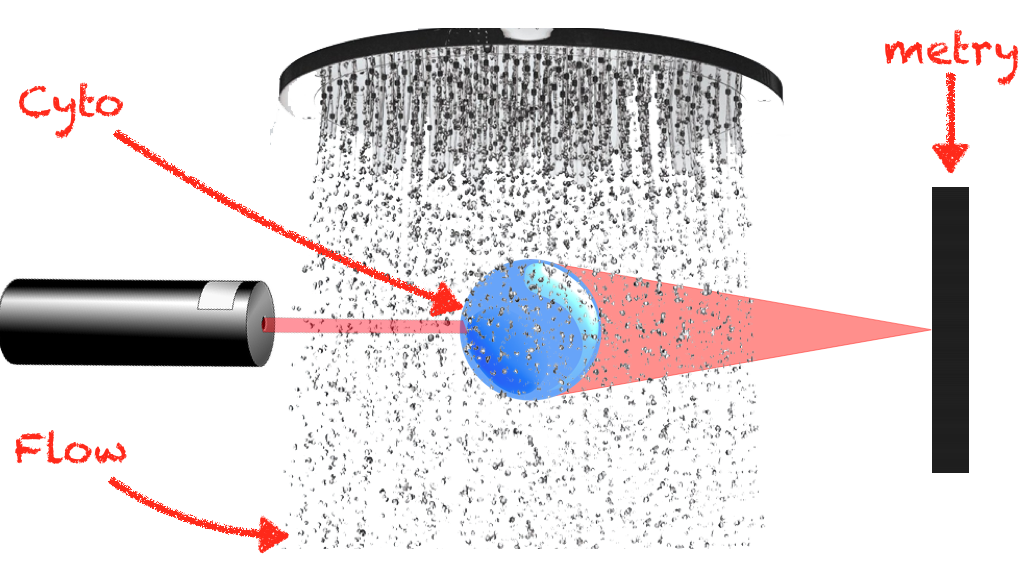
\includegraphics[width=\linewidth]{flowcyto}
\noindent
\textbf{Flow} -- a stream of 'sticky' fluid passing through a flow cytometer \\
\textbf{Cyto} -- the cells suspended in the fluid stream \\
\textbf{metry} -- the measurements are recorded when a cell is excited by a laser beam
\vspace{0.3em}%this can be altered to set vertical spacing
}

\headerbox{Existing Approach}{name = existing, column = 0, below = cytometry}{
\begin{itemize}[leftmargin=*]
	\item Expert-driven approach 
	\item Non-reproducible results
	\item Underlying data structure ignored
	\item Computationally inefficient
\end{itemize}
\noindent
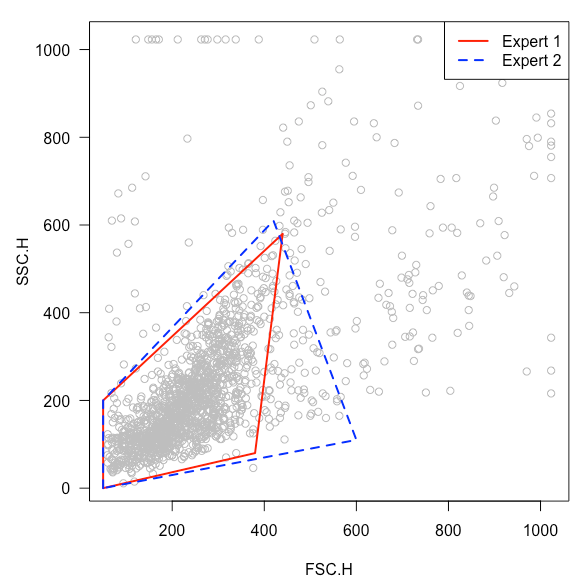
\includegraphics[width=0.95\textwidth]{expertresults}
}

\headerbox{Future Work}{name = future, column = 1, above = bottom, span = 1}{
\vspace{1em}
\noindent
\textbf{Flow Cytometry}
\begin{itemize}[leftmargin=*]
	\item Gating in multiple dimensions
	\item Open Source Software solution
\end{itemize}
\vspace{0.7em}	
\noindent
\textbf{Equity Models}
\begin{itemize}[leftmargin=*]
	\item Pricing of Renewable Feed-In Tariffs
\end{itemize}
\vspace{0.5em} %this can be altered to set vertical spacing
}

%%%%%%%%%%%%%% Finish Column 0 %%%%%%%%%%%%%%%%%%

\headerbox{Probability Map -- Markov Random Fields}{name = mrf, column = 1, span = 2}{
\noindent
\begin{minipage}{\linewidth}
	\begin{minipage}{0.45\linewidth}
		\noindent
		Let $L$ be an $N \times N$ lattice grid where
		{\color{nodered} $$X_{ij} \in \{-1, +1\}$$}
		with each observation $X_{ij}$ having first order neighbours defined by
		{\color{nodeblue}$$\eta_{ij} = \{(\ell,m):0<(i-\ell)^2 + (j - m)^2 \leq 1 \}.$$}
		$L$ is thus a Markov Random Field following a Gibbs Distribution with conditional probability mass function of a single node being defined as
		$$\text{Pr}({\color{nodered}X_{ij} = x_{ij}} | {\color{nodeblue}X_{\ell m} = x_{\ell m}, (\ell,m) \in \eta_{ij}})$$ 
		$$= \frac{\exp\left({\color{nodered} x_{ij}} {\color{nodeblue}\sum\limits_{\eta_{ij}} x_{\ell m} }\right)}{\exp \left({\color{nodeblue}\sum\limits_{\eta_{ij}} X_{\ell m}} \right) + \exp \left( - {\color{nodeblue}\sum\limits_{\eta_{ij}}X_{\ell m}} \right)}$$
	\end{minipage}\hfill
	\begin{minipage}{0.53\linewidth}
		\hfill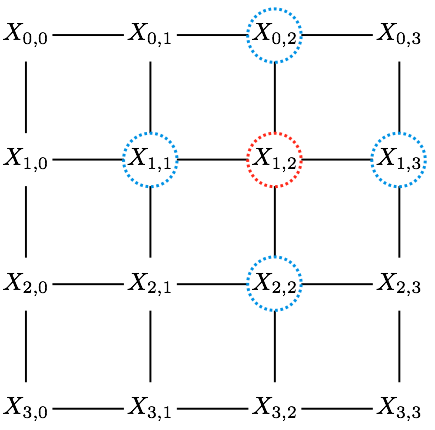
\includegraphics[width=0.95\linewidth]{mrf}
	\end{minipage}
\end{minipage}
\vspace{0.3em}
}

\headerbox{Segmentation -- Connected Components Labelling}{name = cluster, column = 1, span = 2, below = mrf}{
\begin{minipage}{\textwidth}
	\vspace{0.5em}
\end{minipage}

\noindent
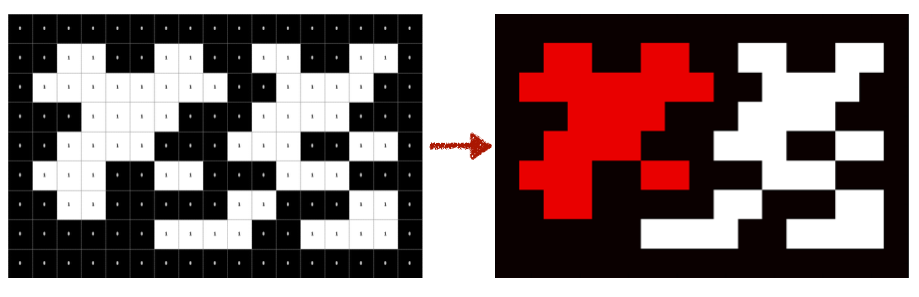
\includegraphics[width=\linewidth]{connectedcomponents}
\begin{minipage}{\linewidth}
	\begin{minipage}{0.48\linewidth}
		\begin{enumerate}[leftmargin=*]
			\item Begin with a realisation of the Markov Random Field Probability Map 
			\item Assign unique labels to each group of pixels \& record label ties
		\end{enumerate}
	\end{minipage}\hfill
	\begin{minipage}{0.48\linewidth}
		\begin{enumerate}[leftmargin=*]\addtocounter{enumi}{2}
			\item Re-assign groups with label ties to lowest group label
			\item Identification of homogeneous regions within the image
		\end{enumerate}
	\end{minipage}
\end{minipage}
\vspace{0.3em}
}

\headerbox{Results}{name = results, column = 1, span = 2, below = cluster}{
\noindent
\begin{minipage}{\textwidth}
	\vspace{0.5em}
\end{minipage}

\noindent
\begin{tabular}{@{\hspace{0.0em}}c@{\hspace{0.75em}} | @{\hspace{0.75em}}c@{\hspace{0.75em}} | @{\hspace{0.75em}} c@{\hspace{0.0em}}}
\textbf{Original Image} & \textbf{MRF Probability Map} & \textbf{Segmentation}\\
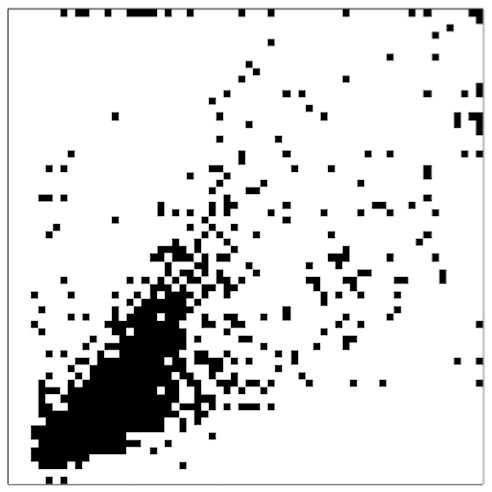
\includegraphics[width=0.31\linewidth]{original} &
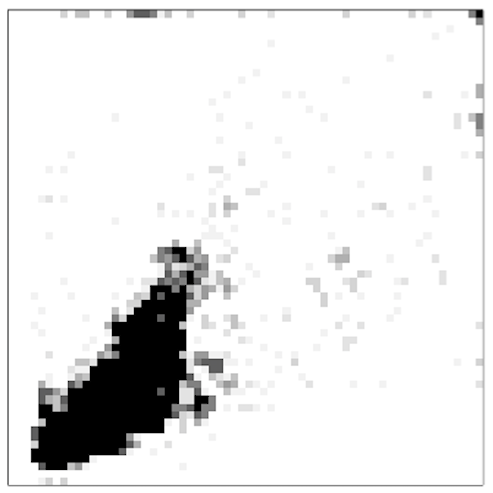
\includegraphics[width=0.31\linewidth]{probmap} &
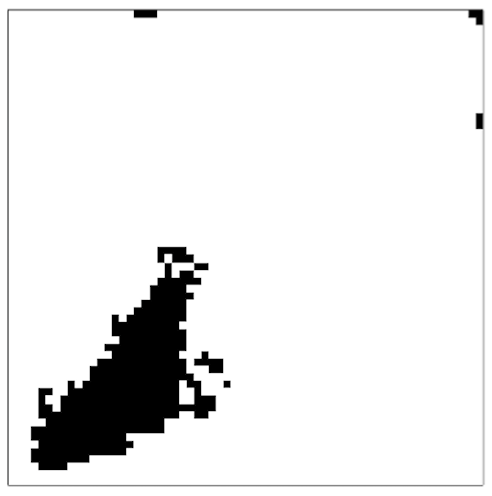
\includegraphics[width=0.31\linewidth]{segmentation} \\
\end{tabular}
\vspace{0.3em}
}

\headerbox{Application Areas}{name = applications, column = 0, above = bottom, span = 1}{
\vspace{0.3em}
\begin{itemize}[leftmargin=*]
	\item Diagnosis and monitoring of leukaemia and lymphoma patients
	\item Quality control in Dairy Sciences 
	\item Food Safety
\end{itemize}
\vspace{0.3em} %this can be altered to set vertical spacing
}

\headerbox{Presentations}{name = pubs_pres, column = 2, above = bottom, span = 1}{
\noindent
\begin{itemize}[leftmargin=*]
	\item Gating of Flow Cytometry Data via Adaptive Markov Random Fields. \textit{Royal Statistical Society Invited Session.} University of Manchester. 8$^{th}$ September 2016.

	\item A Markov Random Fields Approach to the Gating of Flow Cytometry Data. \textit{Research Students Conference in Probability and Statistics.} University College Dublin. 15$^{th}$ June 2016.
\end{itemize}	
\vspace{0.2em} %this can be altered to set vertical spacing
}

\end{poster}
\end{document}